\documentclass{article}
\usepackage[utf8]{inputenc}
\usepackage{amsmath}
\usepackage{natbib}
\linespread{1}
\usepackage{bm}
\usepackage{mcode}
\usepackage[lighttt]{lmodern}
\usepackage{graphicx} 
\usepackage{epstopdf}
\usepackage{algorithm2e}
\usepackage{multicol}
\usepackage{float}
\usepackage{subfigure}
\title{\LARGE{Polymer Chain Dynamics Simulation}\\ \large{Report}
}
\author{ZHA Chenyu}
%\date{5.Mars.2015}
\renewcommand*\contentsname{Table de matière}

\begin{document}

\maketitle
\pagebreak


\section{The random walk model:the freely jointed chain}
\paragraph{}

Consider a linear polymer to be a freely-jointed chain with N beads, length of each bond is $b$ , that occupy zero volume. The path of the chains is like a 'random walk 'in three dimensions, limited only by the constraint that each segment must be joined to its neighbors.\\

Consider the 'end to end' vector $\bm{R}$ joining one end of the polymer to the other,the average value $<\bm{R}>$ is zero,since the probability of R equals -R.Therefore we will calculate $<\bm{R^2}>$
\begin{equation}
<\bm{R^2}>=\sum_{{n=1}}^{N}\sum_{m=1}^{N}<r_n\cdot r_m>
\end{equation} 
We consider that there is no correlation between bead $n$ and $m$,therefore we find :
\begin{equation}
<\bm{R^2}>=\sum_{{n=1}}^{N}<r_n^2>=Nb^2
\end{equation}
The probability distribution of $\bm{R}$ is:
\begin{equation}
P(\bm{R},N)=(\frac{3}{2\pi Nb^2})^{3/2}exp(-\frac{3\bm{R}^2}{2Nb^2})
\end{equation}
The probability distribution function of $\bm{R}$ obeys the Gaussian distribution.
The position of the beads after each step will satisfy the diffusion equation :
\begin{equation}
\bm{R(t+\Delta t)}=\bm{R(t)}+\sqrt{2D\Delta t}\bm{g(t)}
\end{equation}
$\bm{g(t)}$ is normally distributed random noise.
\subsection{Random walk Simulation}
We simulate the random walk with the following parameters :
\begin{lstlisting}
dimension      = 3;;%dimension=1,2 or 3
numParticles   = 100;%number of particles in polymers;
dt             =0.1;%pas de temps
numSteps       =100;% number of motion
diffusionConst =0.1; %constante diffusion
paths          =[];  ; %the paths of polymer;
\end{lstlisting}
The following graph is the trajectory of beads in the first step and last step;
\begin{figure}[H]
	\begin{minipage}[t]{0.5\textwidth}
		\centering
	
		
		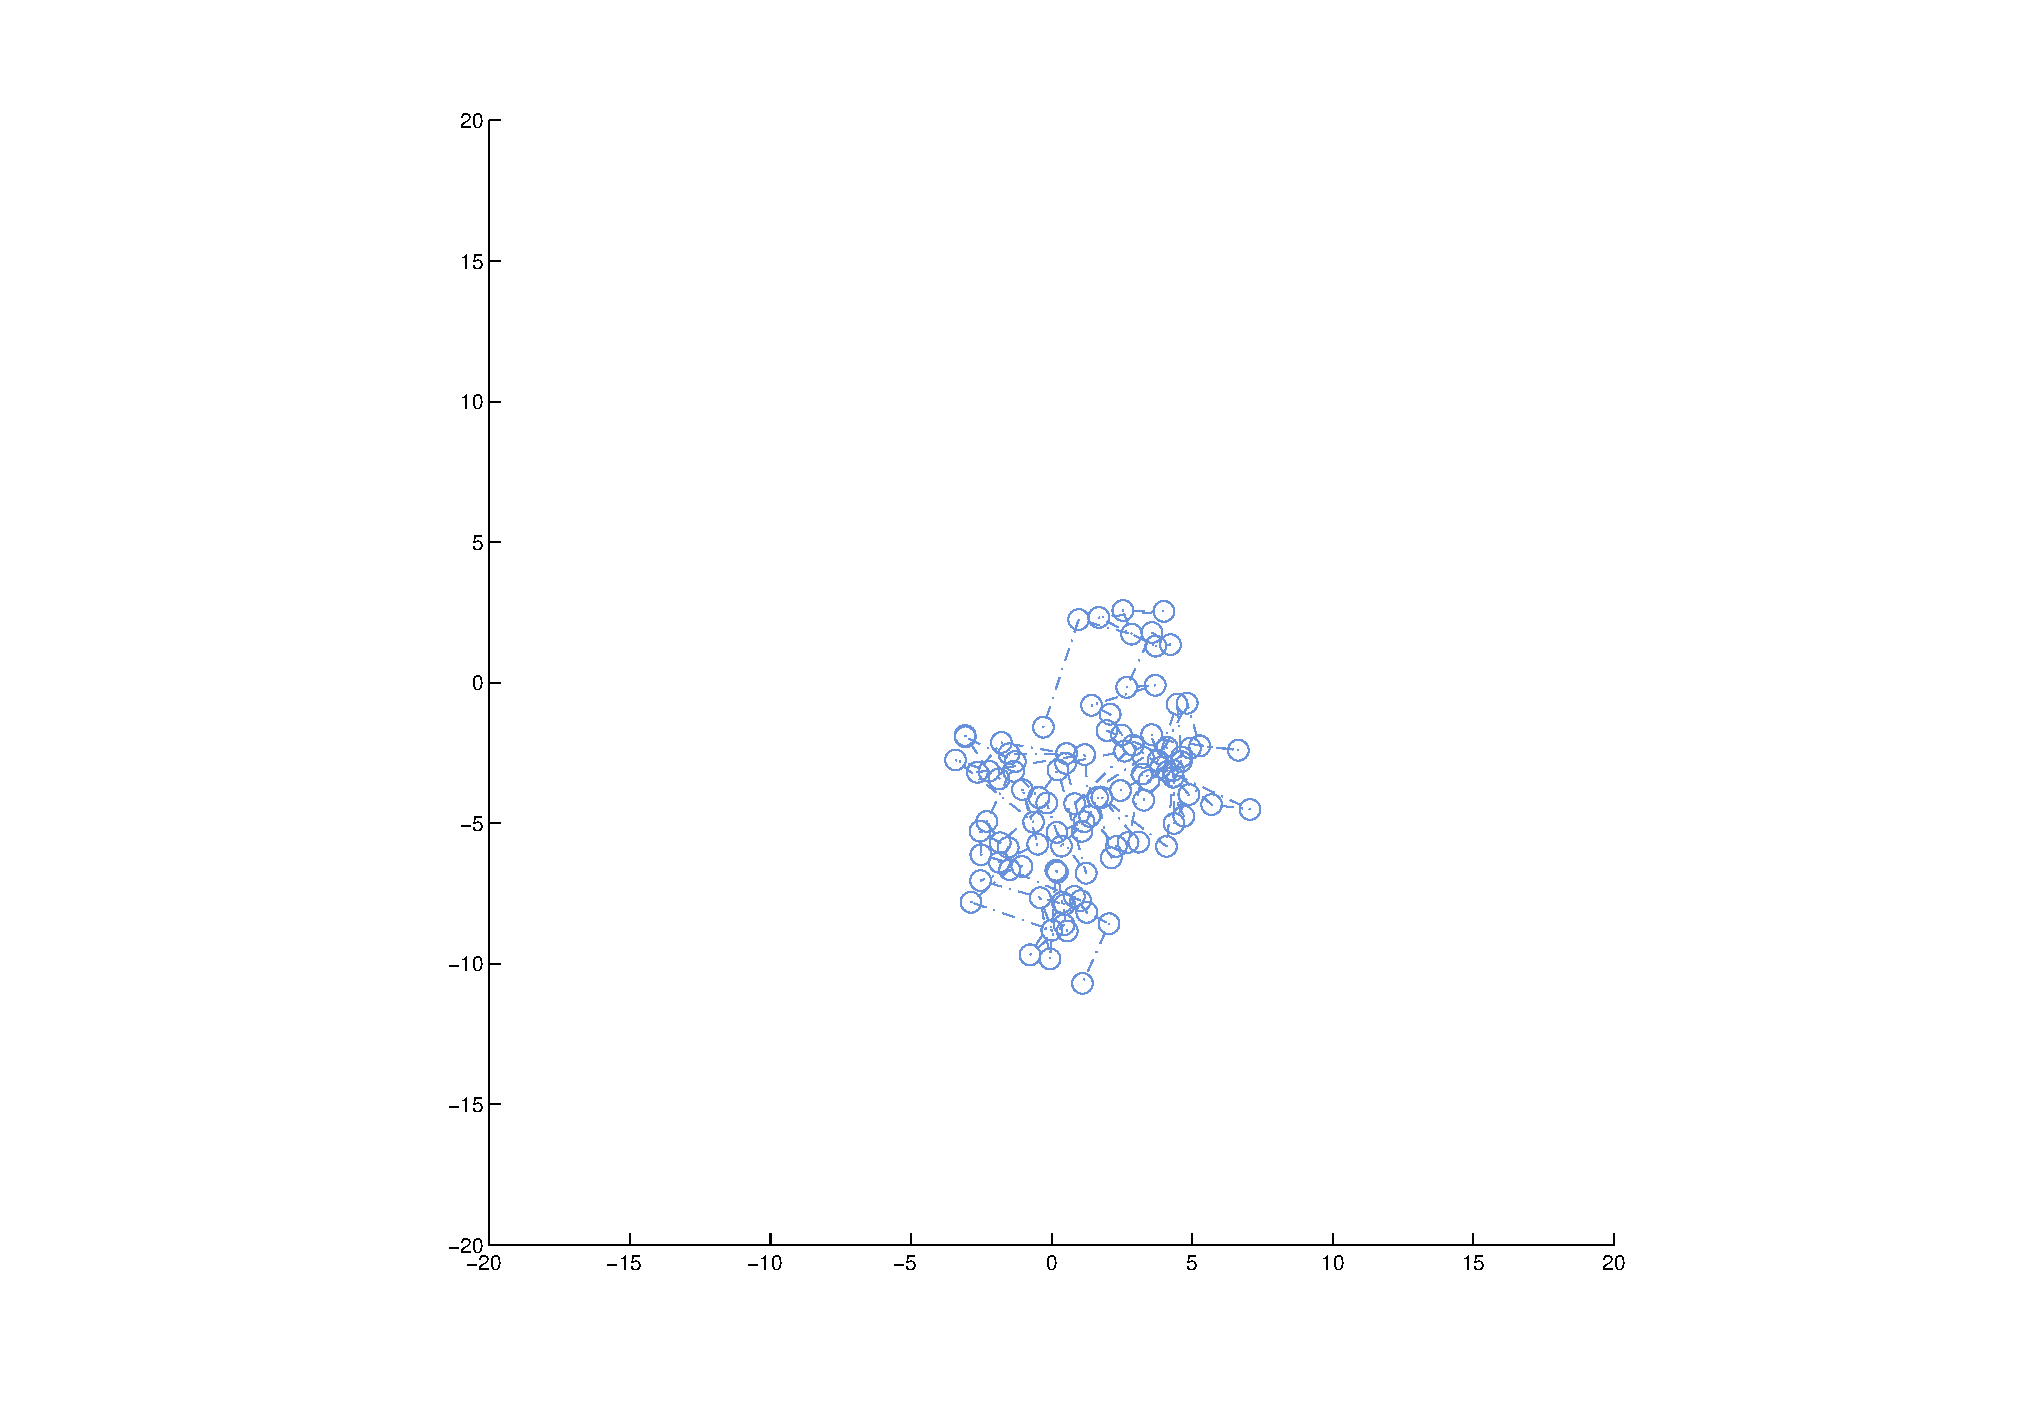
\includegraphics[width=3.2in]{1.eps}
		\caption{initial position}
	\end{minipage}%
	\begin{minipage}[t]{0.5\textwidth}
		\centering
		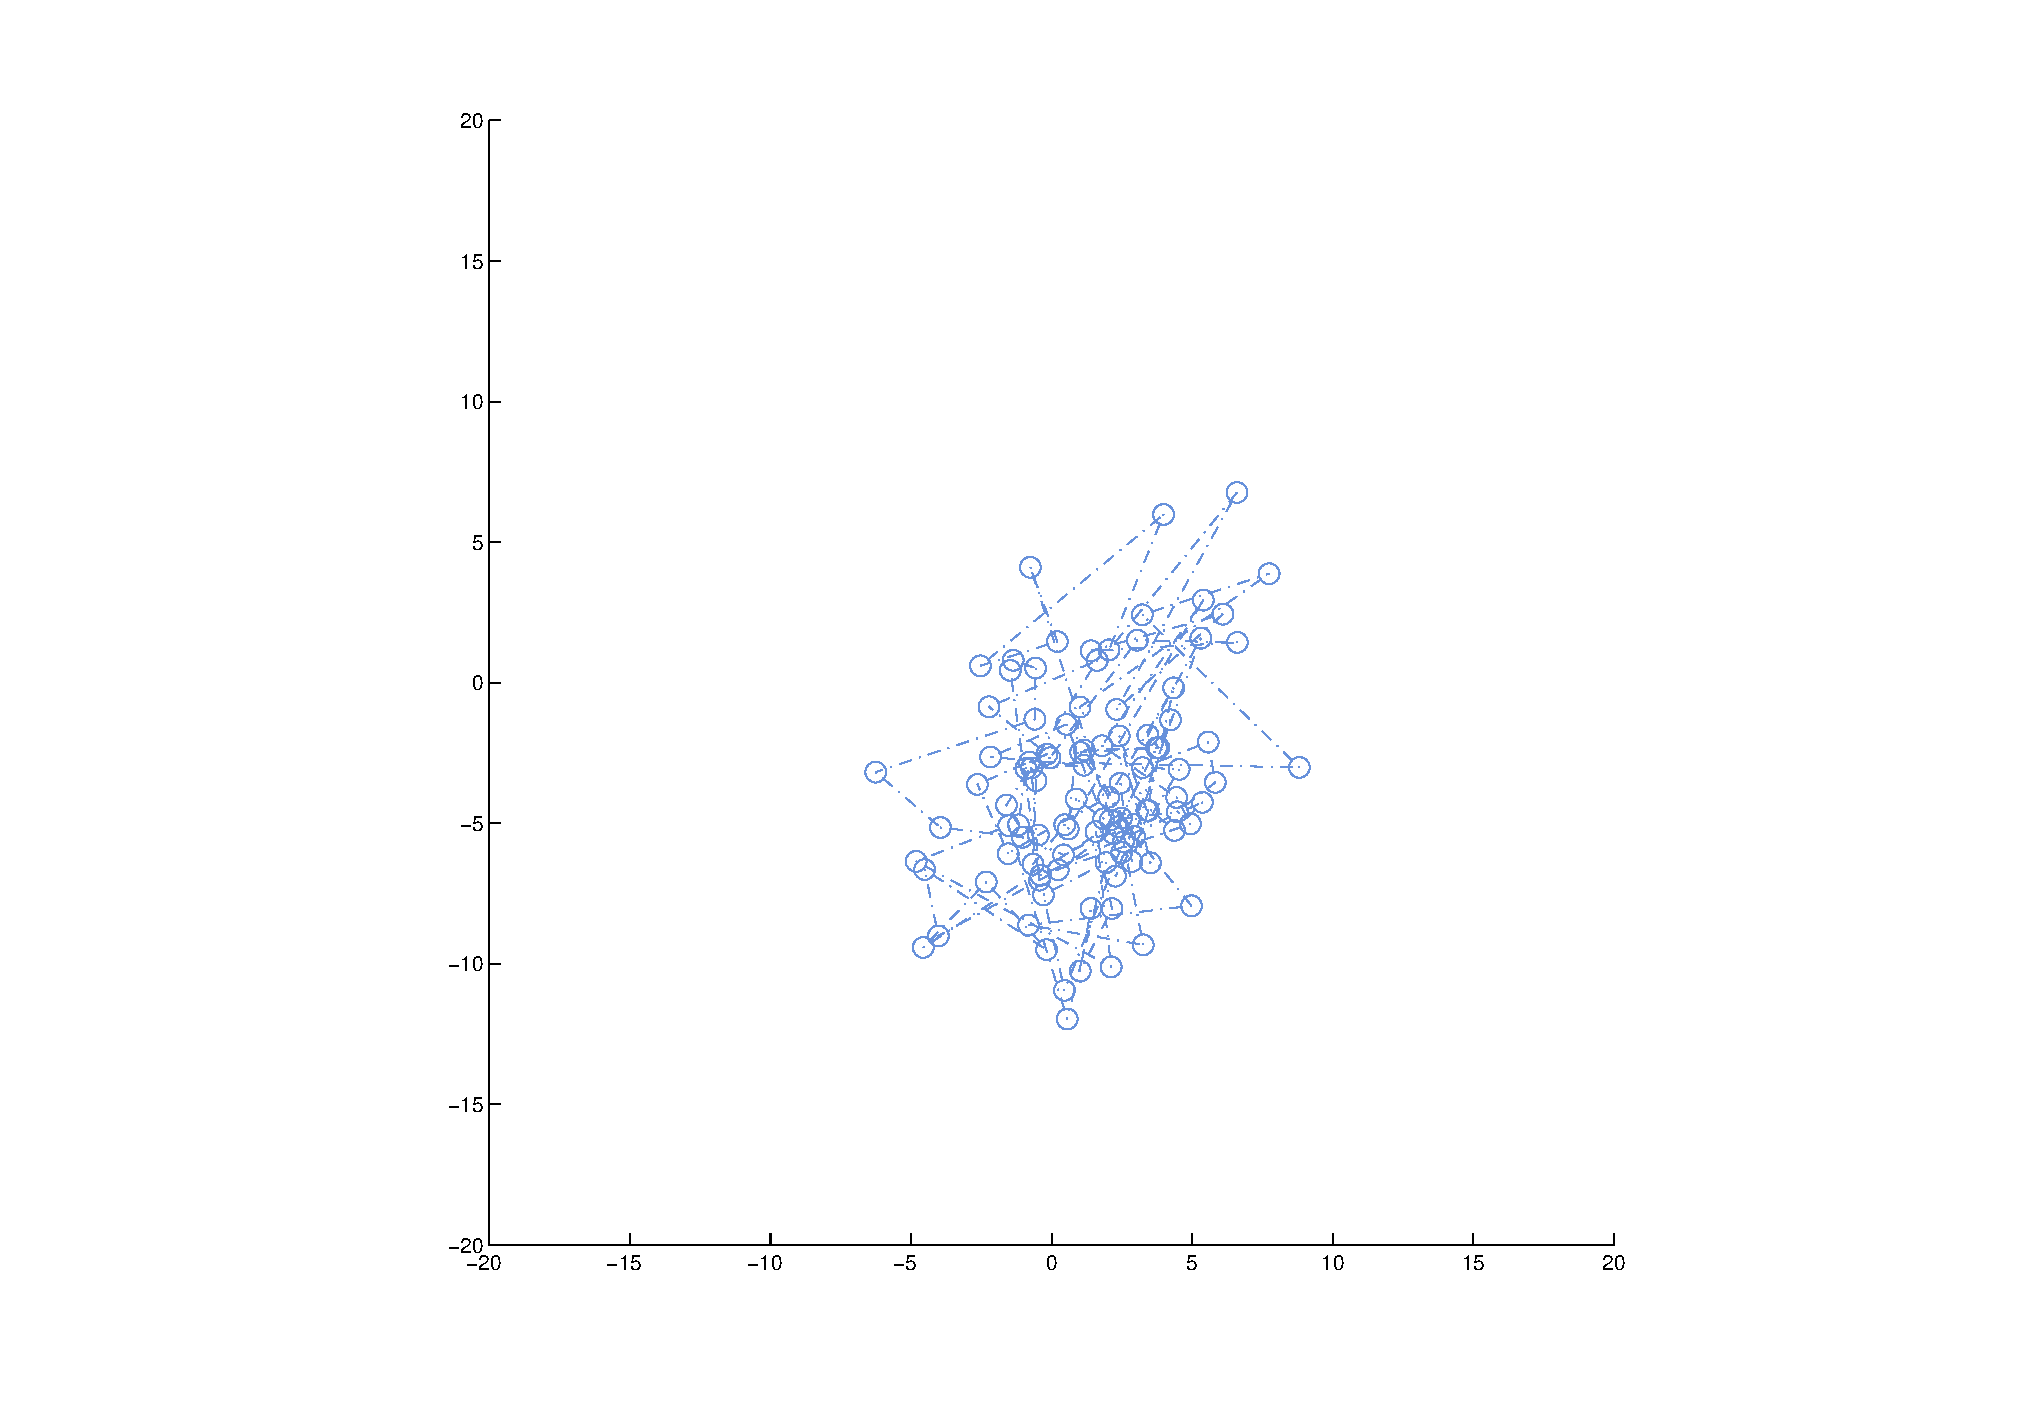
\includegraphics[width=3.2in]{2.eps}
		\caption{final position}
		
	\end{minipage}
\end{figure}
\subsection{Probability density function of $\bm{R}$  }
In order to verify that the PDF of $\bm{R}$ is Gaussian,we calculate the 'end to end distance' $\bm{R}$ for each simulation,then we plot it with histogram by coordinate $(x,y,z)$ respectively and compare with the probability density function of $\bm{R}$ in theory. \\
We simulate the probability density of Gaussian  with the following parameters :
\begin{lstlisting}

     dimension: 3
     numParticles: 100
     dt: 0.1000
     numSteps: 100
     diffusionConst: 0.1000
     paths: [2x3x2 double]
     simulation: 1000

\end{lstlisting}
The following graphs verify that for each coordinate,the distribution of $\bm{R}$ is Gaussian;
\begin{figure}[H]
	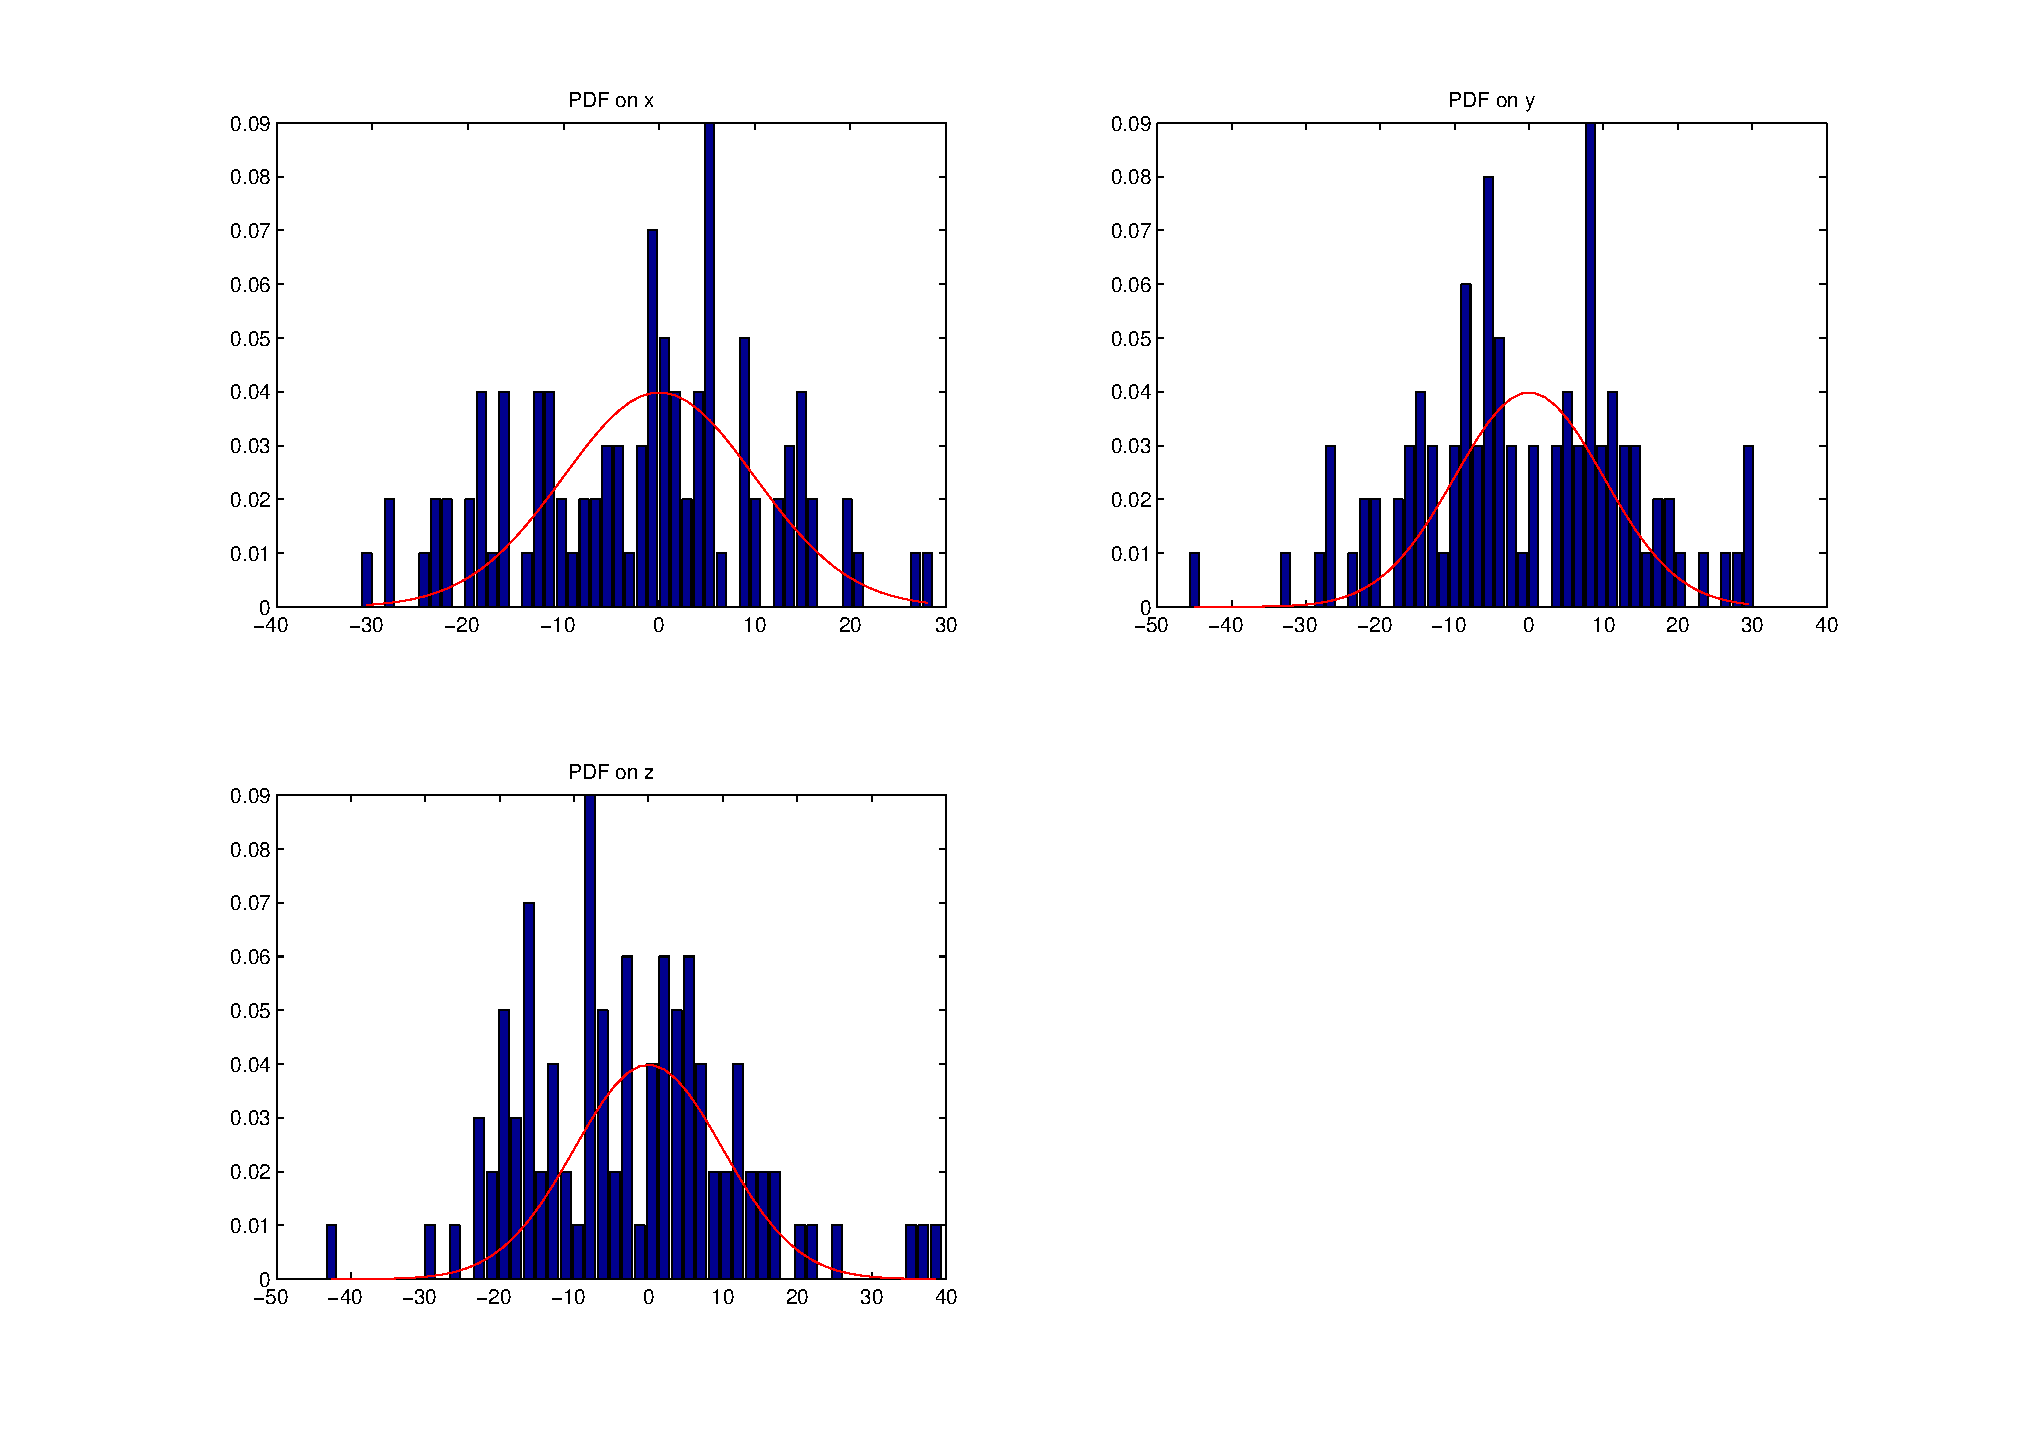
\includegraphics[width=6.2in]{PDF.eps} 
	 
	 \end{figure}
	 \section{The bead-spring model}
	 \paragraph{}
	 The bead-spring model is also called Rouse Model .In this model,the single chain diffusion is represented by Brownian motion ,there is no exclude volume 	interactions between the beads and each bead experience a drag force proportional to their velocity ,then the position of the beads will satisfy the Langevin equation :
	 \begin{equation}
	 \frac{d\bm{R_n}}{dt}=\frac{k}{\xi}(\bm{R_{n+1}}+\bm{R_{n-1}}-2\bm{R_{n}})+\bm{g_n}, \forall n \in [1,2...N-1]
	 \end{equation}
	 For the bead $0$ and $N$,we have :
	 \[
	 \begin{cases}
	\frac{d\bm{R_0}}{dt}=\frac{k}{\xi}(\bm{R_{1}}-\bm{R_{0}})+\bm{g_n}\\
	\frac{d\bm{R_n}}{dt}=\frac{k}{\xi}(\bm{R_{n-1}}-\bm{R_{n}})+\bm{g_n}
	 \end{cases}
	 \]
	 where $\xi$ is friction coefficient,$k$ is spring constant.
	 \subsection{Rouse Model Simulation}
	 We simulate the Rouse Model with the following parameters:
	 \begin{lstlisting}
	  dimension: 3
	  numParticles: 100
	  dt: 0.1000
	  numSteps: 100
	  diffusionConst: 0.1000
	  paths: [100x3x100 double]
	  simulation: 1
	  pathsNormal: [100x3x100 double]
	  frictionCoefficient: 1
	  connectedBeads: []
	  fixedBeads: []
	  b: 1
	 \end{lstlisting}
	 The following graph is the trajectory of beads in the first step and last step;
	 \begin{figure}[H]
	 	\begin{minipage}[t]{0.5\textwidth}
	 		\centering
	 		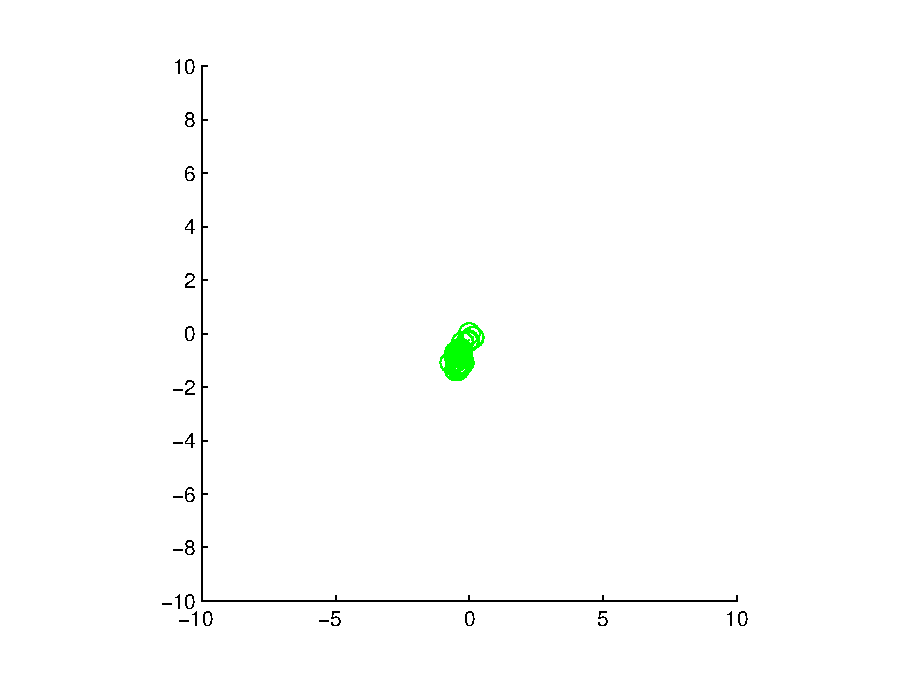
\includegraphics[width=3.2in]{rouseM.eps}
	 		\caption{initial position}
	 	\end{minipage}%
	 	\begin{minipage}[t]{0.5\textwidth}
	 		\centering
	 		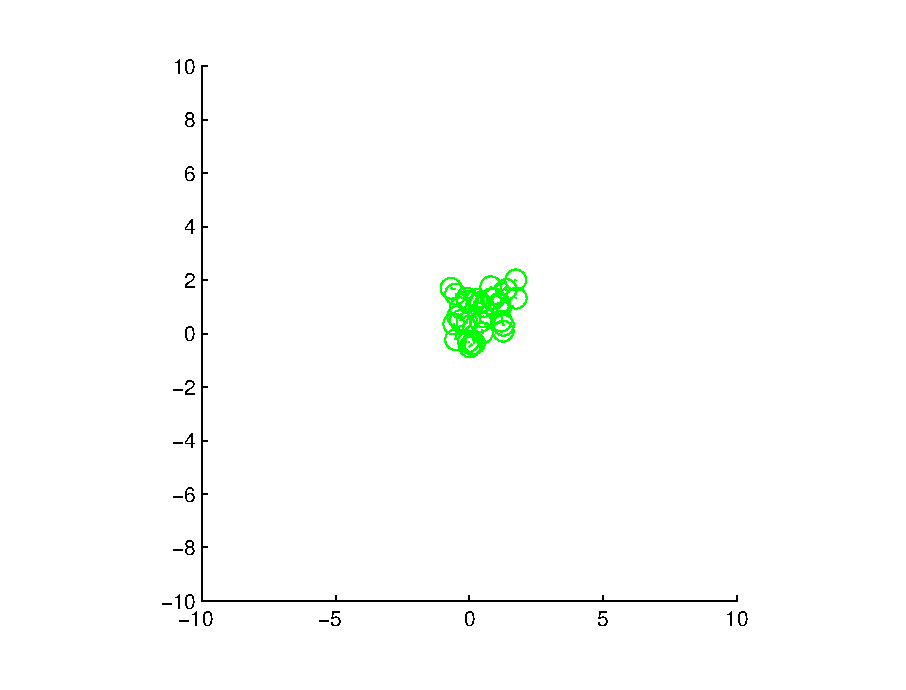
\includegraphics[width=3.2in]{rouseMF.eps}
	 		\caption{final position}
	 		
	 	\end{minipage}
	 \end{figure}
\subsection{Simulation of the mean first-encounter time in the Rouse Model}
\paragraph{}
We want to simulate the mean first-encounter time that 3 beads have met each other in a chain during each simulation, in order to verify that the probability distribution function is exponential.We set 32 beads and we do the simulations with the first bead,last bead ,the third bead we set it from 2 to 16,that means we have $[1,2,32],[1,3,32]...[1,16,32]$ cases.For each case,we calculate the mean first-encounter time and we plot with histogram.

The following parameters are used to simulate the mean first-encounter time:
\pagebreak
\begin{lstlisting}
dimension           = 3;
numParticles        = 32;
dt                  = 0.01;
diffusionConst      = 1;
numSteps            = 100;
numSimulations      = 1000;
frictionCoefficient = 1;
connectedBeads      = [];
fixedBeads          = [];
metBeadNum          = [ones(1,14);[2:15];32*ones(1,14)]';
b                   = 1;
encounterDistance   = b./5;
\end{lstlisting}

\section{Brownian bridge simulation}
The Brownian bridge is a Brownian motion which is starting at $x$ at time $t_0$ and passing through point $y$ at $T$, $T \geq t$,it is defined as :\\
\begin{equation}
B(t) = w(t-t_0)-\frac{t-t_0}{T-t_0}[w(T-t_0)-y+x]+x
\end{equation}
which $w(T)$ is a random walk process.\\
The following steps are used to build a Brownian bridge in domain :\\
1.Initialization of beads on the domain's boundary;\\
2.list all constrain beads in ascending order $c={a_1,a_2,...a_{N_c}}$\\
3.choose a random position for $B_{a_1}$;\\
4.For$i =2...N_c$,choose a position for $B_{a_i}$ by diffusion on the boundary $a_i -a_{i-1}$ steps;\\
5.for all of points in $c$,if $a_{i}-a_{i-1}>1$,construct a Brownian bridge between each 2 points by using the formula above;\\
6.if $a_1 \leq 1$ or $a_{N_c} \geq BeadsEnd,$sequentially build a path form the 1 to $a_1$ and $a_{N_c}$ to $BeadsEnd$.\\
\end{document}